\documentclass[../../../analisi-dei-requisiti.tex]{subfiles}

\begin{document}

\subsubsection{AUC4: Gestione luoghi}%
\label{subs:AUC4}

\begin{figure}[H]
  \centering
  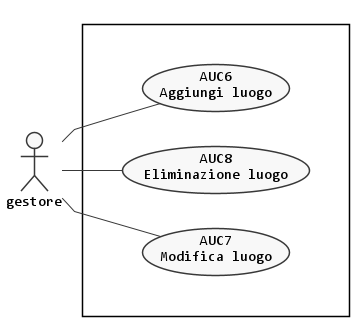
\includegraphics[width=100mm]{gestione-luoghi}
  \caption{AUC4: Gestione luoghi}%
  \label{fig:AUC4}
\end{figure}

\begin{description}
  \item[Codice:] AUC4;
  \item[Titolo:] Gestione luoghi;
  \item[Attori primari:] gestore;
  \item[Precondizione:] il sistema deve rendere disponibile la pagina di gestione dei luoghi di un'organizzazione;
  \item[Postcondizione:] vengono gestiti i luoghi di un'organizzazione;
  \item[Scenario principale:]
  \begin{enumerate}
    \item sorge la necessità di effettuare operazioni sul luogo di un'organizzazione, e viene offerta la possibilità di selezionarlo.
  \end{enumerate}
\end{description}

\subsubsection{AUC4.1: Aggiungi luogo}%
\label{subs:AUC4.1}

\begin{figure}[H]
  \centering
  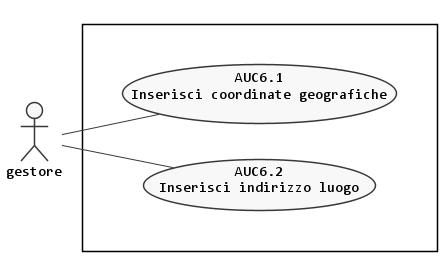
\includegraphics[width=100mm]{aggiungi-luogo.png}
  \caption{AUC4.1: Aggiungi luogo}%
  \label{fig:AUC4.1}
\end{figure}

\begin{description}
  \item[Codice:] AUC4.1;
  \item[Titolo:] Aggiungi luogo;
  \item[Attori primari:] gestore;
  \item[Precondizione:] il \glossario{luogo} da aggiungere nell'organizzazione non deve esistere;
  \item[Postcondizione:] il nuovo luogo viene aggiunto nell'organizzazione;
  \item[Scenario principale:]
  \begin{enumerate}
    \item sorge la necessità di aggiungere un luogo ad un'organizzazione.
  \end{enumerate}
\end{description}

\subsubsection{AUC4.1.1: Inserisci coordinate geografiche}%
\label{subs:AUC4.1.1}
\begin{description}
  \item[Codice:] AUC4.1.1;
  \item[Titolo:] Inserisci coordinate geografiche;
  \item[Attori primari:] gestore;
  \item[Precondizione:] il sistema deve rendere disponibile la possibilità di inserire le coordinate geografiche di un nuovo luogo;
  \item[Postcondizione:] le coordinate geografiche sono inserite correttamente;
  \item[Scenario principale:]
  \begin{enumerate}
    \item l'amministratore inserisce le coordinate geografiche di un nuovo luogo.
  \end{enumerate}
\end{description}

\subsubsection{AUC4.1.2: Inserisci indirizzo luogo}%
\label{subs:AUC4.1.2}
\begin{description}
  \item[Codice:] AUC4.1.2;
  \item[Titolo:] Inserisci indirizzo luogo;
  \item[Attori primari:] gestore;
  \item[Precondizione:] il sistema deve rendere disponibile la possibilità di inserire l'indirizzo di un nuovo luogo;
  \item[Postcondizione:] l'indirizzo è inserito correttamente;
  \item[Scenario principale:]
  \begin{enumerate}
    \item l'amministratore inserisce l'indirizzo di un nuovo luogo.
  \end{enumerate}
\end{description}

\subsubsection{AUC4.2: Eliminazione luogo}%
\label{subs:AUC4.2}
\begin{description}
  \item[Codice:] AUC4.2;
  \item[Titolo:] Eliminazione luogo;
  \item[Attori primari:] gestore;
  \item[Precondizione:] il luogo dell'organizzazione deve essere presente in \emph{Stalker};
  \item[Postcondizione:] il luogo dell'organizzazione viene eliminato;
  \item[Scenario principale:]
  \begin{enumerate}
    \item sorge la necessità di eliminare un luogo di un'organizzazione.
  \end{enumerate}
\end{description}

\subsubsection{AUC4.3: Modifica luogo}%
\label{subs:AUC4.3}

\begin{figure}[H]
  \centering
  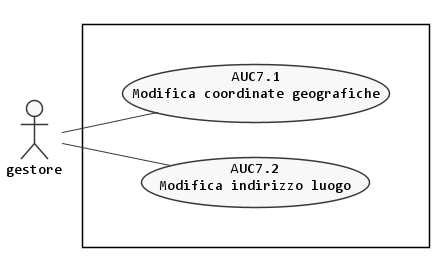
\includegraphics[width=100mm]{modifica-luogo.png}
  \caption{AUC4.3: Modifica luogo}%
  \label{fig:AUC4.3}
\end{figure}

\begin{description}
  \item[Codice:] AUC4.3;
  \item[Titolo:] Modifica luogo;
  \item[Attori primari:] gestore;
  \item[Precondizione:] il luogo dell'organizzazione deve essere presente in \emph{Stalker};
  \item[Postcondizione:] il luogo dell'organizzazione viene modificato;
  \item[Scenario principale:]
  \begin{enumerate}
    \item sorge la necessità di modificare un luogo di un'organizzazione.
  \end{enumerate}
\end{description}

\subsubsection{AUC4.3.1: Modifica coordinate geografiche}%
\label{subs:AUC4.3.1}
\begin{description}
  \item[Codice:] AUC4.3.1;
  \item[Titolo:] Modifica coordinate geografiche;
  \item[Attori primari:] gestore;
  \item[Precondizione:] il sistema deve rendere disponibile la possibilità di modificare le coordinate geografiche di un luogo;
  \item[Postcondizione:] le coordinate geografiche sono state modificate;
  \item[Scenario principale:]
  \begin{enumerate}
    \item l'amministratore vuole modificare le coordinate geografiche di un luogo.
  \end{enumerate}
\end{description}

\subsubsection{AUC4.3.2: Modifica indirizzo luogo}%
\label{subs:AUC4.3.2}
\begin{description}
  \item[Codice:] AUC4.3.2;
  \item[Titolo:] Modifica indirizzo luogo;
  \item[Attori primari:] gestore;
  \item[Precondizione:] il sistema deve rendere disponibile la possibilità di modificare l'indirizzo di un luogo;
  \item[Postcondizione:] l'indirizzo del luogo è stato modificato;
  \item[Scenario principale:]
  \begin{enumerate}
    \item l'amministratore vuole modificare l'indirizzo di un luogo.
  \end{enumerate}
\end{description}
%gestione luoghi (end)

\end{document}
